% --------------------------------------
% Document Class
% --------------------------------------
\documentclass[a4paper,11pt]{article}
% --------------------------------------



% --------------------------------------
% Use Package
% --------------------------------------


\usepackage[francais]{babel}
%\usepackage{ucs}
\usepackage[utf8]{inputenc}
\usepackage[T1]{fontenc}

\usepackage{makeidx}
\usepackage{color}
\usepackage{graphicx}
\usepackage{float}
\usepackage[hidelinks]{hyperref} 
\usepackage{geometry}
%\usepackage{lastpage}
%\usepackage{marginnote}
\usepackage{fancyhdr}
%\usepackage{titlesec}
%\usepackage{framed}
\usepackage{amsmath}
\usepackage{empheq}
\usepackage{array}
\usepackage{multicol}
\usepackage{csquotes}
%\usepackage{adjustbox}

% insert code
\usepackage{listings}

% define our color
\usepackage{xcolor}

% code color
\definecolor{ligthyellow}{RGB}{250,247,220}
\definecolor{darkblue}{RGB}{5,10,85}
\definecolor{ligthblue}{RGB}{1,147,128}
\definecolor{darkgreen}{RGB}{8,120,51}
\definecolor{darkred}{RGB}{160,0,0}

% other color
\definecolor{ivi}{RGB}{141,107,185}


\lstset{
    language=R,
    captionpos=b,
    extendedchars=true,
    frame=lines,
    numbers=left,
    numberstyle=\tiny,
    numbersep=5pt,
    keepspaces=true,
    breaklines=true,
    showspaces=false,
    showstringspaces=false,
    breakatwhitespace=false,
    stepnumber=1,
    showtabs=false,
    tabsize=3,
    basicstyle=\small\ttfamily,
    backgroundcolor=\color{ligthyellow},
    keywordstyle=\color{ligthblue},
    morekeywords={include, printf, uchar},
    identifierstyle=\color{darkblue},
    commentstyle=\color{darkgreen},
    stringstyle=\color{darkred},
}


% --------------------------------------



% --------------------------------------
% Page setting
% --------------------------------------
%\pagestyle{empty}
\setlength{\headheight}{15pt}

\setcounter{secnumdepth}{3}
\setcounter{tocdepth}{2}

\makeatletter
\@addtoreset{chapter}{part}
\makeatother 

\hypersetup{         % parametrage des hyperliens
  colorlinks=true,      % colorise les liens
  breaklinks=true,      % permet les retours à la ligne pour les liens trop longs
  urlcolor= blue,       % couleur des hyperliens
  linkcolor= black,     % couleur des liens internes aux documents (index, figures, tableaux, equations,...)
  citecolor= green      % couleur des liens vers les references bibliographiques
}

% --------------------------------------

% --------------------------------------
% Information
% --------------------------------------
\title{Compte-rendu TP5 RdF : Segmentation automatique par analyse d’histogramme}
\author{Elliot VANEGUE et Gaëtan DEFLANDRE}
% --------------------------------------

\definecolor{myColor}{rgb}{0.5, 0.1, 0.75}

% --------------------------------------
% Begin content
% --------------------------------------
\begin{document}

% Set language to english
  \selectlanguage{francais}

  % Start the page counting
  \pagenumbering{arabic}

  \maketitle
  
  \mbox{}
  \newpage
  \clearpage
  
  \section*{Introduction}
  %Lors de ce TP, nous allons voir comment segmenter une image en niveau de gris en
  %créant des macros avec le langage R. Nous utiliserons le seuillage automatique 
  %de Bayes afin de voir les avantages et les inconvénients de cette méthode.
  
  Lors de ce TP, nous allons voir comment automatiser la segmention d'une image en niveaux de gris en 
  utilisant le théorème de Bayes. Nous créerons des macros en language R 
  afin de voir les avantages et les inconvénients de cette méthode.

  \section{Seuillage fixe}
   
  Dans un premier temps, nous avons testé plusieurs seuils proches sur l'image \\
  \enquote{2classes\_100\_100\_8bits.png}, pour mettre en évidence l'importance de trouver un seuil précis .\\
  
  \begin{figure}[H]
    \center
    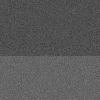
\includegraphics[width=5cm]{2classes_100_100_8bits.png}
    \caption{Image 2classes\_100\_100\_8bits.png}
  \end{figure}
  % Nous voyons que plus nous augmentons le seuil, plus le bruit est important dans la partie basse de l'image. 
  % Inversement, le bruit diminu dans la partie haute de l'image.
  Nous avons pu voir que plus nous augmentons le seuil, plus il y avait de bruit dans l'image
  binarisée sur la partie du bas. Inversement, lorsque nous diminuons le seuil, le bruit 
  se ressent d'avantage sur la partie du haut de l'image.\\
  
  \begin{figure}[H]
    \center
    
\includegraphics[width=3cm]{resultat/bin35.png}
    
\includegraphics[width=3cm]{resultat/bin36.png}
    
\includegraphics[width=3cm]{resultat/bin37.png}
    \caption{Images binarisées avec un seuil de plus en plus grand}
  \end{figure}
  
  Dans nos résultats, nous avons utilisé des seuils correspondant aux valeurs se trouvant dans le creux
  de l'histogramme de l'image que nous utilisons. Cela permet de séparer les deux pics lors de la 
  binarisation.\\
  
  \begin{figure}[H]
    \center
    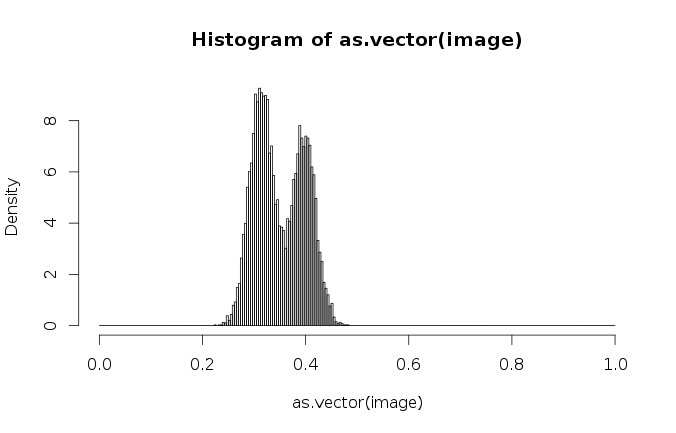
\includegraphics[width=10cm]{resultat/hist_image_principal.png}
    \caption{Histogramme de l'image 2classes\_100\_100\_8bits.png}
  \end{figure}
  
  
  % % Je sais pas, pour moi, on obtiendra le meilleur seuil avec Bayes, 
  % % et de manière automatique. Avec cette méthodes le seui est valide 
  % % que pour une image et c'est pas automatique. Mais je suis pas sur.
  % % Je pense pas que Bayes prend en compte la position et le voisinnage 
  % % des pixels, donc il ne corrigera pas les pixels de trop dans chaque classe.
  %Donc le seuillage en utilisant l'histogramme de gris n'est pas la bonne solution pour 
  %bien classer les pixels de l'image car les deux parties de celle-ci comporte des pixels
  %dont le niveau de gris est similaire.
  Nous pouvons voir que seuiller manuellement une image n'est pas chose facile car il nous
  est impossible d'avoir un bon seuil rien qu'en regardant l'histogramme de gris.
  Nous allons donc voir comment nous pouvons automatiser le seuillage avec le théorème
  de Bayes.
  
  \section{Seuillage automatique (Bayes) - Probabilité a priori des classes}
  Nous allons maintenant calculer la probabilité à priori des deux classes présentes dans l'image
  afin de pouvoir la seuiller grâce à la méthode de Bayes. Nous avons d'abord, besoin de séparer
  les deux classes manuellement pour extraire le nombre de pixels de chacune d'elles, grâce à leur 
  histogramme.\\
  
  \begin{figure}[H]
    \center
    
\includegraphics[width=5cm]{2classes_100_100_8bits_omega1.png}
    
\includegraphics[width=5cm]{2classes_100_100_8bits_omega2.png}
    \caption{Images des classes $\omega_{1}$ (à gauche) et $\omega_{2}$ (à droite)}
  \end{figure}
  
  \begin{figure}[H]
    \center
    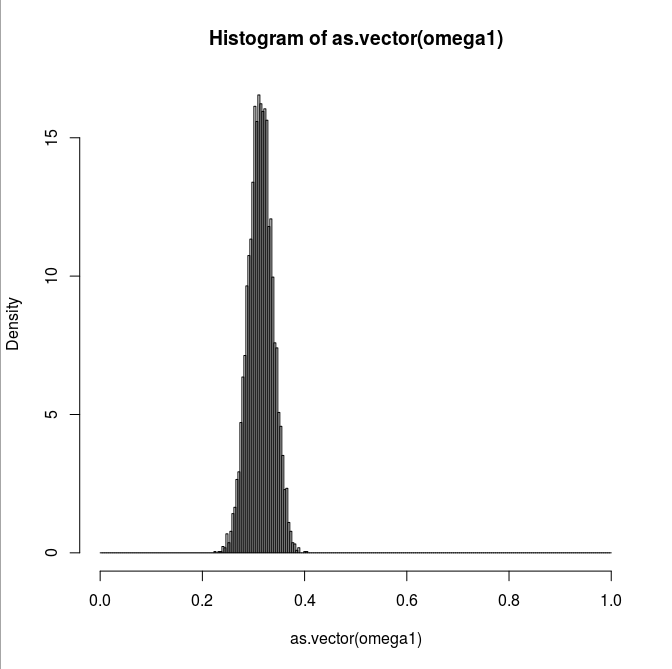
\includegraphics[width=6cm]{resultat/hist_omega1.png}
    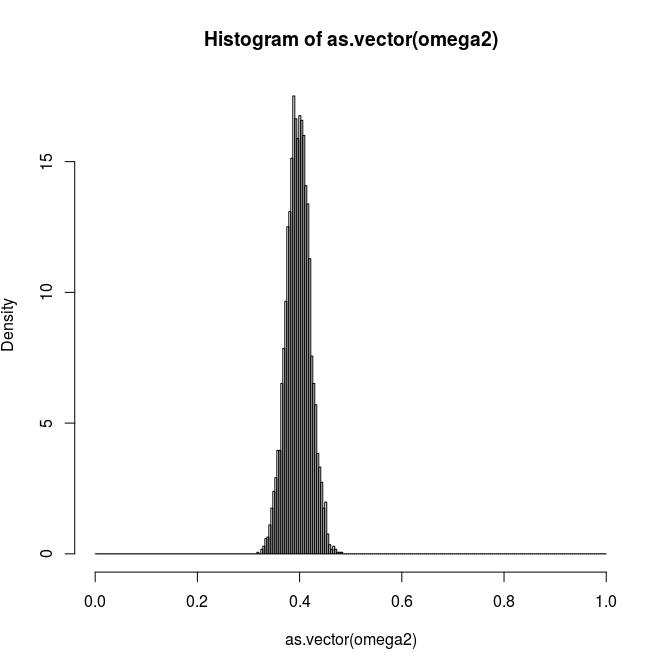
\includegraphics[width=6cm]{resultat/hist_omega2.png}
    \caption{Histogrammes des classes $\omega_{1}$ (à gauche) et $\omega_{2}$ (à droite)}
  \end{figure}
  
  Ensuite, pour calculer cette probabilité, nous divisons le nombre de pixels d'une classe ($N_{\omega_k}$) par
  le nombre total de pixels ($N$). Ce qui nous donne les résultats suivants :
  
  \begin{align*}
    P(\omega_{1}) &= \frac{ N_{\omega_{1}} }{ N } = 0.56 \\
    P(\omega_{2}) &= \frac{ N_{\omega_{2}} }{ N } = 0.44 \\
  \end{align*}
  
  Les macros qui correspondent à ce calcul sont les suivantes :\\
  
  \begin{lstlisting}[caption=Macros de calcule de probabilité à priori des classe $N_{w_1}$ et $N_{w_2}$]
  p_omega1= sum(h1$counts[0:255])/ sum(h$counts[0:255])
  p_omega2= sum(h2$counts[0:255])/ sum(h$counts[0:255])\end{lstlisting}
  
  \section{Seuillage automatique (Bayes) - Probabilité conditionnelle}
  Afin de calculer la probabilité d'erreur, nous avons besoin des probabilités conditionnelles des deux
  classes de l'image pour une valeur donnée. La valeur de X que nous avons utilisé durant nos calculs
  est 79. Nous devons diviser la densité de pixels de gris 79 par la probabilité $P(I)$ pour $P(79/I)$, 
  $P(\omega_1)$ pour $P(79/\omega_1)$ et $P(\omega_2)$ pour $P(79/\omega_2)$. Il faut aussi prendre en compte
  que la densité est en pourcentage et les probabilités sont entre 0 et 1. Ce qui nous donne les résulats suivants :
  %Nous devons diviser le nombre de pixels d'une classe d'un niveau de gris donné par le nombre total de
  %pixels pour obtenir la probabilité conditionnelle. Ce qui nous donne les résulat suivant :
  
  \begin{align*}
    P(79/I) &= \frac{h.density(79)}{100} = 0.092672 \\
    P(79/\omega_1) &= \frac{ h1.density(79) }{ p_{\omega_{1}}*100 } = 0.2955102 \\
    P(79/\omega_2) &= \frac{ h2.density(79) }{ p_{\omega_{2}}*100 } = 0 \\
  \end{align*}
  
  
  %$$P(79/I) = \frac{h(79)}{N} = 0.0362$$
  %$$P(79/w_1) = \frac{h1(79)}{N} = 0.0362$$
  %$$P(79/w_2) = \frac{h2(79)}{N} = 0$$\\
  
  Soit les macros suivantes : \\
  
  \begin{lstlisting}[caption=Macros de calcule de probabilités conditionnelles]
  X = 80;# gris à 79

  p79_I  = h$density[X] / 100
  p79_o1 = h1$density[X] / (p_omega1*100)
  p79_o2 = h2$density[X] / (p_omega2*100)\end{lstlisting}
  
  Nous obtenons donc la probabilité qu'un pixel est de niveau de gris X sachant sa classe.
  
  %\begin{lstlisting}[caption=Macros de calcule de probabilité à priori des classe $N_{w_1}$ et $N_{w_2}$]
  %pI = h$counts[80] / sum(h$counts[0:255])
  %pw1 = h1$counts[80] / sum(h$counts[0:255])
  %pw2 = h2$counts[80] / sum(h$counts[0:255])
  %\end{lstlisting}

  
  %TODO explication resultat 
  \section{Seuillage automatique (Bayes) - probabilité d’erreur}
  Nous allons maintenant trouver le seuil qui propose un taux d'erreur minimum en utilisant 
  les probabilités d'erreurs. Le meilleur seuil est celui pour lequel la probabilité 
  d'erreurs est minimale pour la classe $\omega_1$ et $\omega_2$. Ceci permet une 
  automatisation du seuillage. Néanmoins il nous faut extraire les classes avant de pouvoir 
  faire ce calcul.\\
  
  Pour cela nous utilisons la macro suivante :
  
  \begin{lstlisting}[caption=Macro qui recherche le seuil avec le taux d'erreur minimum]
  # recherche du minimum
  minimum_erreur = 1;
  seuil_minimum_erreur = 0;

  for (X in 1:255) { 
      somme1[X+1] = sum( h1$density[(X+1):256]) / sum(h1$density[1:256] )
    
      somme2[X+1] = sum( h2$density[1:(X+1)]) / sum(h2$density[1:256] )
      somme2[X+1] = somme2[X+1] * p_omega2

      erreur[X+1] = somme1[X+1] + somme2[X+1]
      
      # seuil corrrespondant à l'erreur minimale
      if (erreur[X+1] < minimum_erreur ) seuil_minimum_erreur = X
      if (erreur[X+1] < minimum_erreur ) minimum_erreur = erreur[X+1]
  }
  print(paste("Seuil erreur minimum: ", seuil_minimum_erreur, ""))
  print(paste("Taux d'erreur: ", minimum_erreur, ""))\end{lstlisting}
  
  Nous obtenons le seuil de 92, en valeur de gris, afin de garantir un taux d'erreur minimal 
  de 4,71\%. 
  
  \begin{figure}[H]
    \center
    
\includegraphics[width=3cm]{resultat/binBayes.png}
    \caption{Images binarisées avec un seuil optimal (Bayes).}
  \end{figure}
  
  \section{Extraction de la région représentant le 0 par seuillage automatique (Bayes)}
  
  Pour conserver des informations cohérentes sur les différentes classes liées au chiffre 0,
  il ne faut pas tenir compte des pixels noirs. Ces pixels noirs font partis du fond et 
  n'appartiennent pas aux classes $\omega_1$ et $\omega_2$.
  
  \begin{figure}[H]
    \center
    \shortstack{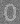
\includegraphics[width=3.0cm]{rdf-chiffre-0-8bits.png} \\ Image source}
    \shortstack{
\includegraphics[width=3.0cm]{rdf-chiffre-0-8bits_omega1.png} \\ Image $\omega_1$}
    \shortstack{
\includegraphics[width=3.0cm]{rdf-chiffre-0-8bits_omega2.png} \\ Image $\omega_2$}
    \caption{Image et classes du chiffre 0}
  \end{figure}
  
  Pour ne pas tenir compte des pixels de fond, il suffit de les annuler, avec les 
  opérations suivantes en R:
  
  \begin{lstlisting}[caption=Annuler les pixels de fond]
  h1$count[1] = 0;
  h1$density[1] = 0.0;
  
  h2$count[1] = 0;
  h2$density[1] = 0.0;
  \end{lstlisting}
  
  \begin{figure}[H]
    \center
    
\includegraphics[width=3cm]{resultat/binZeroBayes.png}
    \caption{Image binarisée du chiffre 0}
  \end{figure}
  
  \section{Seuillage automatique (Bayes) - Segmentation d’une image à 3 classes}
 
  Nous allons maintenant essayer de seuiller une image contenant 3 classes. Comme pour précédemment,
  nous allons utiliser une image par classe afin de segmenter l'image.
  
  \begin{figure}[H]
    \center
    \shortstack{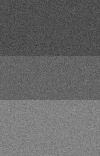
\includegraphics[width=3.5cm]{3classes_100_156_8bits.png} \\ Image source}
    \shortstack{
\includegraphics[width=3.5cm]{3classes_100_156_8bits_omega1.png} \\ Image $\omega_1$}
    \shortstack{
\includegraphics[width=3.5cm]{3classes_100_156_8bits_omega2.png} \\ Image $\omega_2$}
    \shortstack{
\includegraphics[width=3.5cm]{3classes_100_156_8bits_omega3.png} \\ Image $\omega_3$}
    \caption{Images et classes du rectangle à 3 classes}
  \end{figure}
  
  Pour segmenter une image à 3 classes, nous répétons la probabilité d'erreur deux fois. Une première fois
  pour connaitre le seuil entre les classes 1 et 2, et une seconde fois pour le seuil des classes entre 2 et 3.
  Nous obtenons ainsi les valeurs suivantes :
  
  \begin{center}
  \begin{tabular}{|c|c|c|}
   \hline
   classes & seuil d'erreur minimum & taux d'erreur \\
   \hline
   entre les classes $w_1$ et $w_2$ & 92 & 0.030 \\
   \hline
   entre les classes $w_2$ et $w_3$ & 116 & 0.007 \\
   \hline
  \end{tabular}
  \end{center}
  \ \\
  Grâce à ces résultats, nous allons pouvoir segmenter notre image. Pour cela nous allons parcourir l'ensemble 
  des pixels de l'image. Lorsque la valeur d'un pixel dépasse le premier seuil que nous avons déterminé, nous allons 
  mettre la valeur de ce pixel à 127, et lorsque la valeur du pixel dépasse le second seuil, on le met à 255. Tous 
  les autres pixels seront à 0. Cela nous donne le code suivant :\\ 
  
  \begin{lstlisting}[caption=Segmenter une image à trois classe]
  binaire_Bayes = (image*0)

  for (y in 1:height) {
      for (x in 1:width) {
          if(image[x,y]>seuil_1_2){
              binaire_Bayes[x,y] = 0.5
          }
          if(image[x,y]>seuil_2_3){
              binaire_Bayes[x,y] = 1
          }
      }
  }
  \end{lstlisting}
  
  \begin{figure}[H]
    \center
    \includegraphics[width=3.5cm]{resultat/3classesBin.png}
    \caption{Seuillage du rectangle avec deux seuils (Bayes)}
  \end{figure}
  
%   \section{Taux d’erreur de classification}
%   Pour calculer le taux d'erreur d'une segmentation à trois classe, il nous faut soustraire le résultat
%   précédent à l'image d'origine. Puis il faut diviser le cumule des pixels de 1 à 256 par le cumule des pixels
%   de 2 à 256. Ce qui nous donne la macro suivante :\\
%   
  
  
  \section*{Conclusion}
  % Le problème avec Bayes c'est qu'on a besoin de connaitre l'histogramme de chacune des classes, donc pas très pratique.
  Nous avons pu voir que le théorème de bayes est très efficace pour segmenter automatiquement une image. Cependant, il nécessite
  l'histogramme des différentes classes d'une image, ce qui n'est pas toujours fourni.
    
\end{document}  